%%%%%%%%%%%%%%%%%%%%%%%%%%%%%%%%%%%%%%%%%
% Beamer Presentation
% LaTeX Template
% Version 1.0 (10/11/12)
%
% This template has been downloaded from:
% http://www.LaTeXTemplates.com
%
% License:
% CC BY-NC-SA 3.0 (http://creativecommons.org/licenses/by-nc-sa/3.0/)
%
%%%%%%%%%%%%%%%%%%%%%%%%%%%%%%%%%%%%%%%%%

%----------------------------------------------------------------------------------------
%   PACKAGES AND THEMES
%----------------------------------------------------------------------------------------

\documentclass{beamer}

\mode<presentation> {

% The Beamer class comes with a number of default slide themes
% which change the colors and layouts of slides. Below this is a list
% of all the themes, uncomment each in turn to see what they look like.

%\usetheme{default}
%\usetheme{AnnArbor}
%\usetheme{Antibes}
%\usetheme{Bergen}
%\usetheme{Berkeley}
%\usetheme{Berlin}
%\usetheme{Boadilla}
%\usetheme{CambridgeUS}
%\usetheme{Copenhagen}
%\usetheme{Darmstadt}
%\usetheme{Dresden}
%\usetheme{Frankfurt}
%\usetheme{Goettingen}
%\usetheme{Hannover}
%\usetheme{Ilmenau}
%\usetheme{JuanLesPins}
%\usetheme{Luebeck}
\usetheme{Madrid}
%\usetheme{Malmoe}
%\usetheme{Marburg}
%\usetheme{Montpellier}
%\usetheme{PaloAlto}
%\usetheme{Pittsburgh}
%\usetheme{Rochester}
%\usetheme{Singapore}
%\usetheme{Szeged}
%\usetheme{Warsaw}

% As well as themes, the Beamer class has a number of color themes
% for any slide theme. Uncomment each of these in turn to see how it
% changes the colors of your current slide theme.

%\usecolortheme{albatross}
%\usecolortheme{beaver}
%\usecolortheme{beetle}
%\usecolortheme{crane}
%\usecolortheme{dolphin}
%\usecolortheme{dove}
%\usecolortheme{fly}
%\usecolortheme{lily}
%\usecolortheme{orchid}
%\usecolortheme{rose}
%\usecolortheme{seagull}
%\usecolortheme{seahorse}
%\usecolortheme{whale}
%\usecolortheme{wolverine}

%\setbeamertemplate{footline} % To remove the footer line in all slides uncomment this line
%\setbeamertemplate{footline}[page number] % To replace the footer line in all slides with a simple slide count uncomment this line

%\setbeamertemplate{navigation symbols}{} % To remove the navigation symbols from the bottom of all slides uncomment this line
}

\usepackage{algorithm, algorithmic}
\usepackage{booktabs} % Allows the use of \toprule, \midrule and \bottomrule in tables
\usepackage{caption}
\usepackage{ctex}
\usepackage{graphicx} % Allows including images
\usepackage{mathtools}
\usepackage{subcaption}


\newcommand{\tabitem}{%
  \usebeamertemplate{itemize item}\hspace*{\labelsep}}
\newtheorem{remark}[theorem]{Remark}

%----------------------------------------------------------------------------------------
%   TITLE PAGE
%----------------------------------------------------------------------------------------

\title[Short title]{Design and Implementation of Automated Grammar Transformation and Parser Generators\\文法自动变换及解析器生成器的设计与实现} % The short title appears at the bottom of every slide, the full title is only on the title page

\author{Yihan Zhang\\张艺瀚} % Your name
\institute[NEU] % Your institution as it will appear on the bottom of every slide, may be shorthand to save space
{
Northeastern University \\ % Your institution for the title page
\medskip
\textit{zhng1573@hotmail.com} % Your email address
}
\date{\today} % Date, can be changed to a custom date

\begin{document}

\begin{frame}
\titlepage % Print the title page as the first slide
\end{frame}

\begin{frame}
\frametitle{Overview} % Table of contents slide, comment this block out to remove it
\tableofcontents % Throughout your presentation, if you choose to use \section{} and \subsection{} commands, these will automatically be printed on this slide as an overview of your presentation
\end{frame}

\section{文法自动变换}
\subsection{预备知识与记号}
\begin{frame}
\frametitle{预备知识与记号}
\begin{definition}
A context-free grammar(上下文无关文法) $G$ is a quadruple(四元组) $G=(V,T,P,S)$, where $V$ is nonterminal(variable,非终结符号或变元) set, $T$ is terminal(终结符号) set, $P$ is production(产生式) set with productions shaped like $A\to \alpha, A\in V, \alpha\in (V\cup T)^*$, $S$ is start variable(开始变元).
\end{definition}
\end{frame}

\subsection{迭代到不动点}
\begin{frame}
\frametitle{迭代到不动点}
In this frame, we will introduce a technique called "iteration to a fixed point(迭代到不动点)". Take computing the generating symbols(可产生的符号) as an example. A symbol is said to be generating if $A\xRightarrow[]{*} \omega, \omega\in T^*$. In most textbooks, generating symbols are generally computed by the following rules:
\begin{itemize}
\item All terminals are generating;
\item If $A\to \alpha\in P$, $\alpha=\varepsilon$ or every symbol in $\alpha$ is generating. Then $A$ is generating.
\end{itemize}
\end{frame}

\begin{frame}
Given any system of set equations, it's easy to get corresponding algorithm using the technique iteration to a fixed point. Algorithm for the last example is:
\begin{algorithm}[H]
\begin{algorithmic}[1]

\REQUIRE $G=(V,T,P,S)$
\ENSURE $V_{old}=\emptyset, V_{new}=\{ A:A\to\omega\in P,\omega\in T^* \}$

\WHILE{$V_{old}\neq V_{new}$}
\STATE $V_{old}=V_{new}$
\STATE $V_{new}=V_{old}\cup\{ A:A\to\alpha\in P, \alpha\in(T\cup V_{old})^* \}$
\ENDWHILE

\STATE $V=V_{new}$

\end{algorithmic}
\caption{Compute generating variables}
\label{alg:generating}
\end{algorithm}
\end{frame}

\section{解析器生成器}
\subsection{CYK算法及其改进}
\begin{frame}
\frametitle{原始CYK算法}
\begin{algorithm}[H]
\begin{algorithmic}[1]

\REQUIRE $G=(V,T,P,S)$ in CNF, $a_1a_2\cdots a_n\in T^n$

\FOR{$i=0$ \TO $n-1$}
\STATE $ T_{i0}=\{ A:A\to a_i\in P \} $
\ENDFOR

\FOR{$j=1$ \TO $n-1$}
	\FOR{$i=0$ \TO $n-j-1$}
		\STATE $ T_{ij}=\emptyset $
		\FOR{$k=0$ \TO $j-1$}
			\STATE $ T_{ij}=T_{ij}\cup\{ A:A\to BC\in P, B\in T_{ik}, C\in T_{(i+k)(j-k)} \} $
		\ENDFOR
	\ENDFOR
\ENDFOR

\end{algorithmic}
\caption{Original CYK}
\label{alg:original_cyk}
\end{algorithm}
\end{frame}

\begin{frame}
\begin{remark}
CYK algorithm requires the input grammar to be in CNF(乔姆斯基范式), whose productions are all in the form $A\to BC, B, C\in V$. Definition of $T_{ij}$ in the algorithm is $T_{ij}=\{ A: A\xRightarrow[]{*}a_ia_{i+1}\cdots a_{i+j-2}a_{i+j-1} \}$. After running the algorithm, if $S\in T_{1n}$, then $a_1a_2\cdots a_n\in L(G)$.
\end{remark}
\end{frame}

\begin{frame}
\frametitle{改进CYK算法}
\begin{algorithm}[H]
\begin{algorithmic}[1]

\ENSURE $M=$ all \FALSE, $M[0,i,j]=$\TRUE, $i=0,1,\cdots,n,V_j\to a_i\in P$

\FOR{$i=1$ \TO $n-1$}
	\FOR{$j=0$ \TO $n-i-1$}
		\FOR{$k=0$ \TO $i-1$}
			\FORALL{$V_A\TO V_BV_C$}
				\IF{$M[k,j,B],M[i-k-1,j+k+1,C]$}
					\STATE $M[i,j,A]=$\TRUE
				\ENDIF
			\ENDFOR
		\ENDFOR
	\ENDFOR
\ENDFOR

\end{algorithmic}
\caption{Improved CYK}
\label{alg:improved_cyk}
\end{algorithm}
\end{frame}

\begin{frame}
\begin{remark}
After running the improved version, if $M[n-1,0,S]$, then $V_S\in T_{1n}$. In fact, $V_k\in T[i,j] \iff M[i,j,k]$. Considering $V$ is a finite set, we use a 3-dimensional boolean matrix(三维布尔矩阵) $M$ to represent whether a variable is in an entry of the original 2-dimensional variable-set matrix(二维变元集合矩阵) $T$. This improvement avoids union-find operation of sets(集合的并查操作) which may have a high-complexity implementation and makes the algorithm more practical.
\end{remark}
\end{frame}

\subsection{Earley算法及其改进}
\begin{frame}
\frametitle{原始Earley算法}
Given any augmented CFG(增广文法,with additional variable $S'$ and production $S'\to S$) $G$ and $a_1a_2\cdots a_n\in T^n$, Earley algorithm maintains a list of $n+1$ sets and can be divided into two stages:
\begin{enumerate}
\item Initialization(初始化): $S_0=\{(S'\to\cdot S, 0) \} $;
\item Assuming the current position is in the $k$-th slot of input string, perform the following operation until a fixed point:
\begin{itemize}
\item Predict(预测) $S_k$;
\item Scan(扫描) $S_k$;
\item Complete(扩充) $S_k$.
\end{itemize}
\end{enumerate}
\end{frame}

\begin{frame}
\frametitle{改进Earley算法}
\begin{algorithm}[H]
\caption{Earley}
\label{fig: earley}

\begin{algorithmic}[1]

\FOR{$k = 0$ \TO $n$}
\FORALL{$ s\in S_k $}
\IF{$\cdot$ is at the end}
\IF{nonterminal after $\cdot$}
\STATE{Predict$(G, k, s)$}
\ELSE
\STATE{Scan$(a_1a_2\cdots a_n, k, s)$}
\ENDIF
\ELSE
\STATE{Complete$(k, s)$}
\ENDIF
\ENDFOR
\ENDFOR
\end{algorithmic}
\end{algorithm}
\end{frame}

\begin{frame}
\begin{remark}
The improved version modifies three operations to make them act on a single state rather than a state set and puts them into a wider loop, reducing repeated search(减少重复搜索).
\end{remark}
\end{frame}

\section{系统设计}
 \begin{frame}
 \frametitle{系统设计}
\begin{figure}
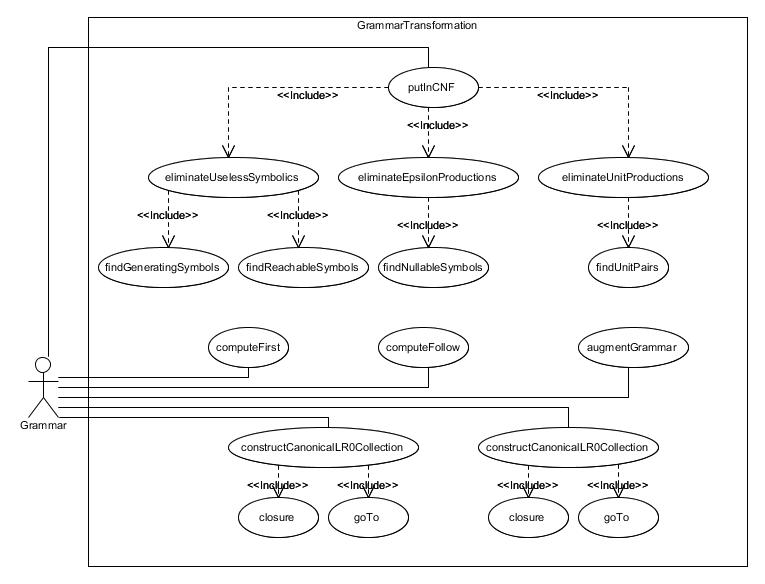
\includegraphics[height=0.75\textheight]{GrammarTransformation.jpg}
\caption{文法自动变换用例图}
\label{fig: gt}
\end{figure}
 \end{frame}
 
  \begin{frame}
\begin{figure}
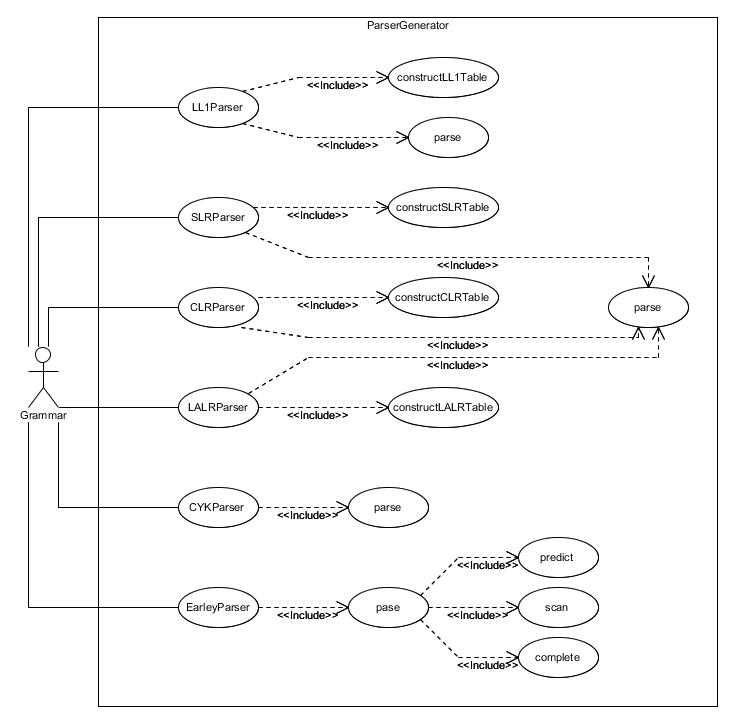
\includegraphics[height=0.8\textheight]{ParserGenerators.jpg}
\caption{解析器生成器用例图}
\label{fig: pg}
\end{figure}
 \end{frame}
 
   \begin{frame}
\begin{figure}
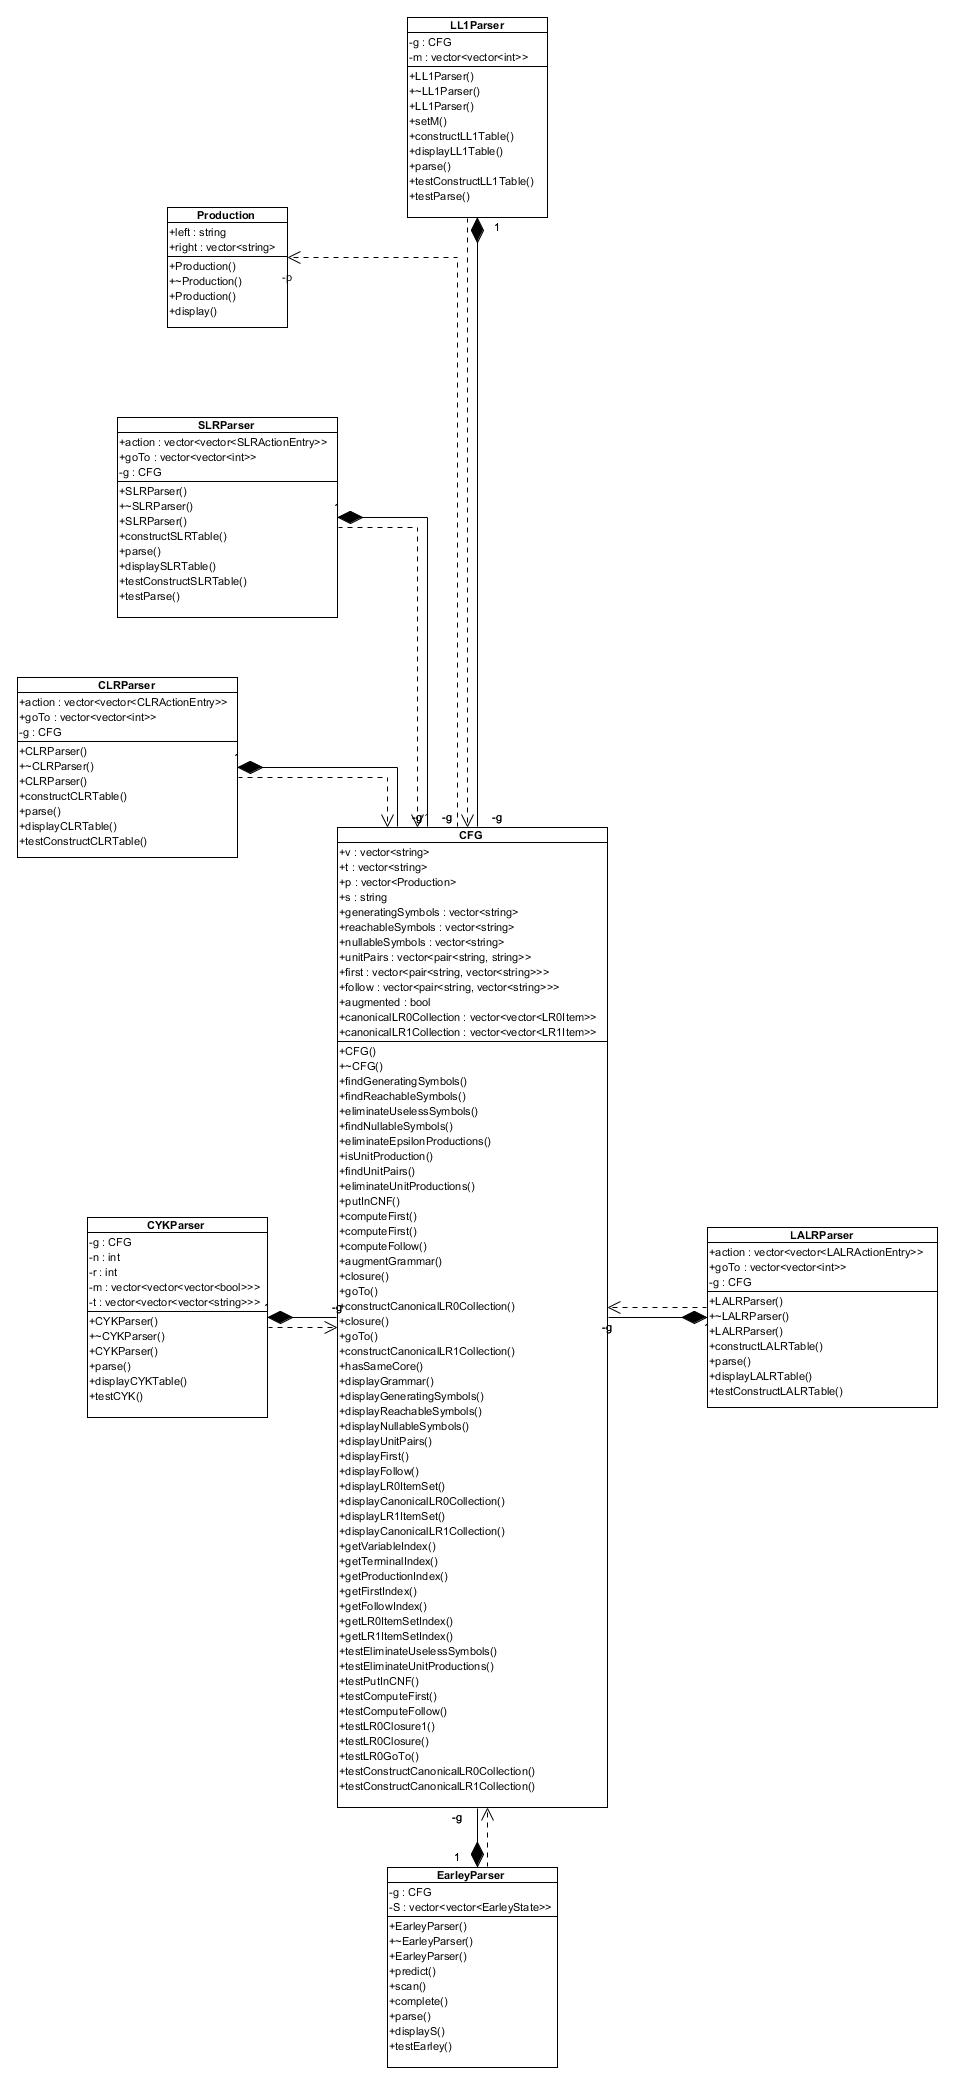
\includegraphics[height=0.8\textheight]{ClassDiagram.jpg}
\caption{类图}
\label{fig: class}
\end{figure}
 \end{frame}
 
 \begin{frame}
      Automated grammar transformer(simplify any given CFG and compute relevant sets automatically,文法自动变换:自动化简任意CFG并计算相关集合): 
      \begin{itemize}
      \item Eliminate useless symbols(去除无用符号); 
      \item Eliminate $\varepsilon$-productions(去除$\varepsilon$-产生式); 
     \item Eliminate unit production(去除单一产生式); 
      \item Put in CNF(化为乔姆斯基范式). 
      \end{itemize}
     
     Parser generators(generate parse table for any given CFG automatically,解析器生成器:自动生成任意CFG的语法分析表): 
     \begin{itemize}
\item CYK, Earley 
\item LL(1) 
\item SLR, CLR, LALR
    \end{itemize}
  
 \end{frame}

\section{系统实现}
 \begin{frame}
 \frametitle{系统实现}
 \begin{itemize}
 \item Hardware:ThinkPad-Edge-E530, 3.5GiB memory, Intel Core i5-3210M CPU, 2.50GHzx4, Intel Ivybridge Mobile;
 \item Operating system: Ubuntu 14.04 LTS, 64-bit;
 \item Tools: C++1y, Sublime Text 3, makefile;
 \item Environment requirement: g++ (Ubuntu 4.8.4-2ubuntu1~14.04.1), Copyright (C) 2013 Free Software Foundation, Inc.
 \end{itemize}
 \end{frame}

\section{系统测试}
 \begin{frame}
\begin{figure}
    \centering
    \begin{subfigure}[b]{0.5\textwidth}
        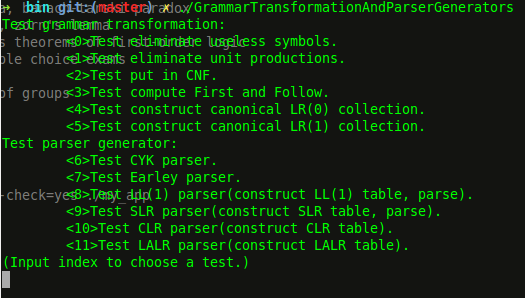
\includegraphics[width=\textwidth]{ui.png}
        \caption{User interface}
        \label{fig:ui}
    \end{subfigure}
    ~ %add desired spacing between images, e. g. ~, \quad, \qquad, \hfill etc. 
      %(or a blank line to force the subfigure onto a new line)
    \begin{subfigure}[b]{0.5\textwidth}
        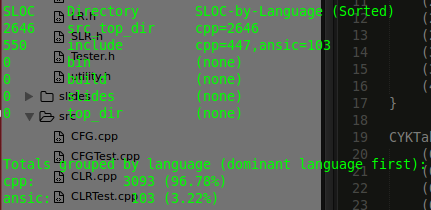
\includegraphics[width=\textwidth]{codes.png}
        \caption{3000+ lines codes}
        \label{fig:codes}
    \end{subfigure}
\end{figure}
 \end{frame}

   \begin{frame}
\begin{figure}
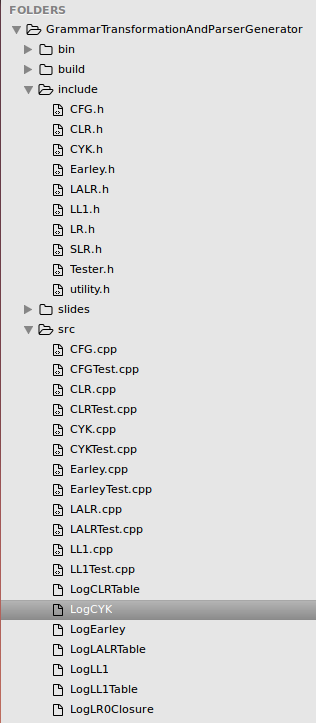
\includegraphics[height=0.8\textheight]{dir.png}
\caption{Directory structure}
\label{fig: dir}
\end{figure}
 \end{frame}

 \begin{frame}
   \frametitle{系统测试}
\begin{figure}
    \centering
    \begin{subfigure}[b]{0.3\textwidth}
        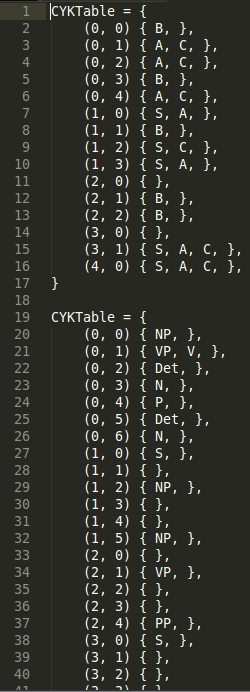
\includegraphics[height=0.75\textheight]{LogCYK.png}
        \caption{CYK log}
        \label{fig:cyk}
    \end{subfigure}
    ~ %add desired spacing between images, e. g. ~, \quad, \qquad, \hfill etc. 
      %(or a blank line to force the subfigure onto a new line)
    \begin{subfigure}[b]{0.3\textwidth}
        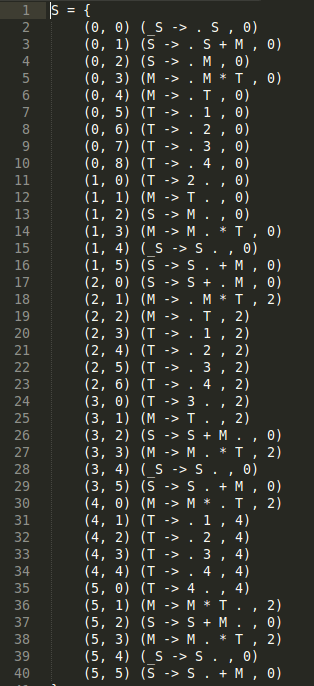
\includegraphics[height=0.75\textheight]{LogEarley.png}
        \caption{Earley log}
        \label{fig:earley}
    \end{subfigure}
\end{figure}
 \end{frame}

  \begin{frame}
\begin{figure}
    \centering
    \begin{subfigure}[b]{0.3\textwidth}
        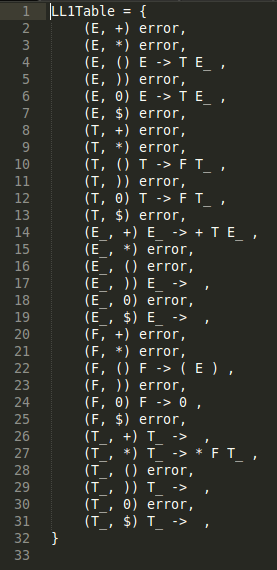
\includegraphics[height=0.8\textheight]{LogLL1Table.png}
        \caption{LL(1) table log}
        \label{fig:ll1table}
    \end{subfigure}
    ~ %add desired spacing between images, e. g. ~, \quad, \qquad, \hfill etc. 
      %(or a blank line to force the subfigure onto a new line)
    \begin{subfigure}[b]{0.3\textwidth}
        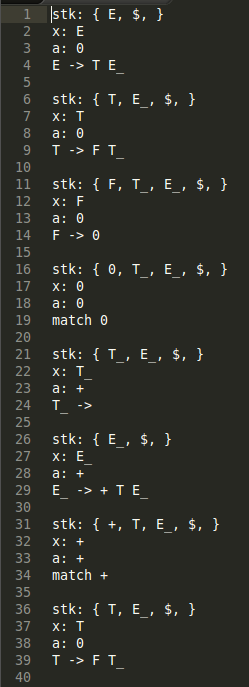
\includegraphics[height=0.8\textheight]{LogLL1.png}
        \caption{LL(1) parsing log}
        \label{fig:ll1}
    \end{subfigure}
\end{figure}
 \end{frame}

\begin{frame}
\begin{figure}
    \centering
    \begin{subfigure}[b]{0.3\textwidth}
        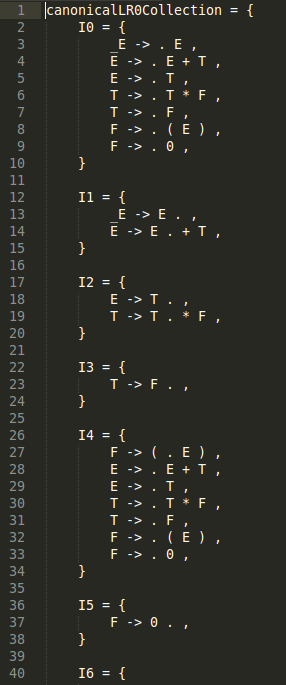
\includegraphics[height=0.8\textheight]{LogLR0Collection.png}
        \caption{LR(0) collection log}
        \label{fig:lr0collection}
    \end{subfigure}
    ~ %add desired spacing between images, e. g. ~, \quad, \qquad, \hfill etc. 
      %(or a blank line to force the subfigure onto a new line)
    \begin{subfigure}[b]{0.3\textwidth}
        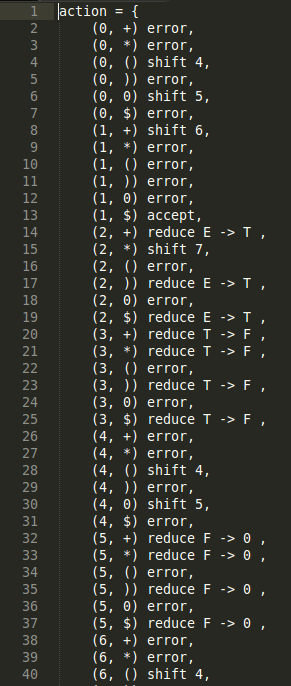
\includegraphics[height=0.8\textheight]{LogSLRTable.png}
        \caption{SLR table log}
        \label{fig:slrtable}
    \end{subfigure}
\end{figure}
\end{frame}

\begin{frame}
\begin{figure}
    \centering
    \begin{subfigure}[b]{0.3\textwidth}
        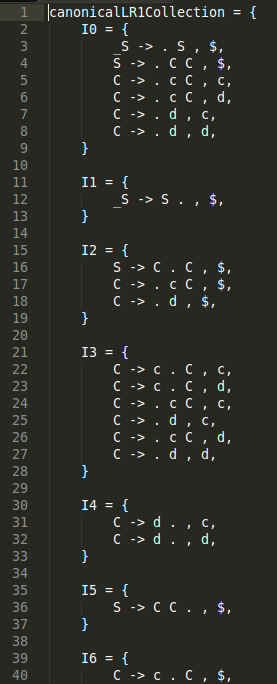
\includegraphics[height=0.8\textheight]{LogLR1Collection.png}
        \caption{LR(1) collection log}
        \label{fig:lr1collection}
    \end{subfigure}
    ~ %add desired spacing between images, e. g. ~, \quad, \qquad, \hfill etc. 
      %(or a blank line to force the subfigure onto a new line)
    \begin{subfigure}[b]{0.3\textwidth}
        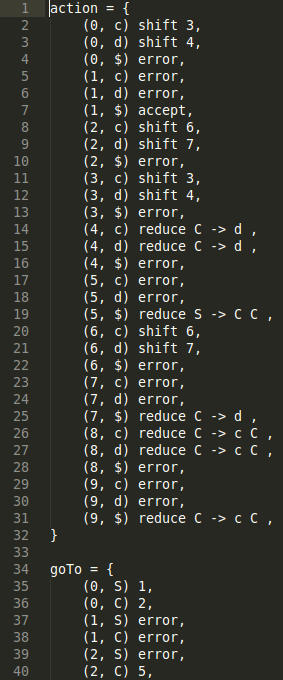
\includegraphics[height=0.8\textheight]{LogCLRTable.png}
        \caption{CLR table log}
        \label{fig:clrtable}
    \end{subfigure}
    ~ %add desired spacing between images, e. g. ~, \quad, \qquad, \hfill etc. 
      %(or a blank line to force the subfigure onto a new line)
    \begin{subfigure}[b]{0.3\textwidth}
        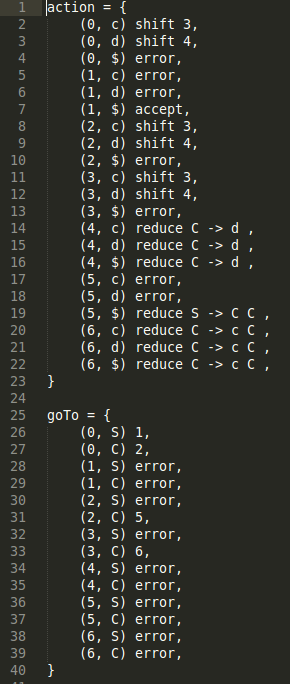
\includegraphics[height=0.8\textheight]{LogLALRTable.png}
        \caption{LALR table log}
        \label{fig:lalrtable}
    \end{subfigure}
\end{figure}
\end{frame}

\section{结论}
 \begin{frame}
 \frametitle{结论}
 We design a C-like grammar(类C文法) which supports most basic syntax of C and use (part of) it to test the system. Conclusions are shown below:
\begin{itemize}
\item Any grammar which $L(G)\backslash\{\varepsilon\}\neq \emptyset$ can be put in CNF;
\item Complexity of CYK and Earley are both $O(n^3)$, while $O(n^2)$ for Earley when handling unambiguous grammars(无二义性文法);
\item Construction of parser generators(解析器生成器) is equivalent to construction of parse tables(语法分析表);
\item LL(1) parser is equivalent to recursive descent parser without backtrack(无回溯递归下降语法分析器);
\item Range of applicable grammars: $\mathrm{SLR}\subset\mathrm{LALR}\subset\mathrm{CLR} $, scale of generated parse tables: $\mathrm{SLR}=\mathrm{LALR}<\mathrm{CLR} $.
\end{itemize}
 \end{frame}

%------------------------------------------------



%------------------------------------------------

\begin{frame}
\Huge{\centerline{Q \& A}}
\end{frame}

%----------------------------------------------------------------------------------------

\end{document}
